% NLP1 Project 1, group 24: six slides with the structure of slides_overleaf.pdf, drawn as figures.
% Build: tectonic slides_figures.tex   (or pdflatex slides_figures.tex)
\documentclass[t,aspectratio=169,10pt]{beamer}

\usepackage[T1]{fontenc}
\usepackage{lmodern}
\usepackage{amssymb}
\usepackage{booktabs}
\usepackage{array}
\usepackage{tikz}
\usetikzlibrary{arrows.meta,positioning,calc,plotmarks}

% ---------- palette ----------
\definecolor{ink}{HTML}{1F2937}
\definecolor{muted}{HTML}{6B7280}
\definecolor{accent}{HTML}{1D4ED8}
\definecolor{neg}{HTML}{C2410C}
\definecolor{pos}{HTML}{0F766E}
\definecolor{amber}{HTML}{B7791F}
\definecolor{panel}{HTML}{F3F4F6}
\definecolor{rule}{HTML}{D1D5DB}

% ---------- theme ----------
\usetheme{default}
\renewcommand{\familydefault}{\sfdefault}
\setbeamertemplate{navigation symbols}{}
\setbeamercolor{normal text}{fg=ink}
\setbeamercolor{structure}{fg=accent}
\setbeamersize{text margin left=9mm,text margin right=9mm}
\setlength{\parskip}{0pt}

\setbeamertemplate{frametitle}{%
  \nointerlineskip\vskip2.6mm
  {\Large\bfseries\color{ink}\insertframetitle}\par\vskip0.4mm
  {\color{accent}\rule{\textwidth}{0.7pt}}\vskip0.8mm}
\setbeamertemplate{footline}{%
  \hbox to\paperwidth{\hspace{9mm}{\color{muted}\tiny NLP1 group 24}%
  \hfill{\color{muted}\tiny \insertframenumber/\inserttotalframenumber}\hspace{9mm}}\vskip2.6mm}

\tikzset{
  every picture/.style={font=\scriptsize,>={Stealth[length=1.6mm]}},
  ttl/.style={anchor=base west,inner sep=0,font=\footnotesize\bfseries},
  note/.style={inner sep=1pt,font=\tiny,text=muted},
  chip/.style={draw=rule,fill=panel,rounded corners=1.5pt,inner sep=2pt,font=\tiny,minimum height=3.6mm},
  ours/.style={chip,draw=accent,fill=accent!10},
}
\newcommand{\lab}[1]{\textcolor{muted}{#1}}
% takeaway bar, always at the same place at the bottom of the slide
\newcommand{\takeaway}[1]{%
  \begin{tikzpicture}[remember picture,overlay]
    \node[anchor=south,fill=accent!7,text width=\dimexpr\paperwidth-18mm-5mm\relax,inner sep=2.5mm,align=left,font=\scriptsize,text=ink]
      (bar) at ([yshift=7.5mm]current page.south) {#1};
    \fill[accent] (bar.north west) rectangle ([xshift=0.8mm]bar.south west);
  \end{tikzpicture}}
\newcommand{\tsep}{\;\textcolor{muted}{$\cdot$}\;}
\newcommand{\num}[1]{\textcolor{accent}{#1}\;}   % panel number
% one stacked posterior bar: x, y, width, half height, P(A better), P(tie)
\newcommand{\postbar}[6]{%
  \fill[ink!55]    (#1,{#2+#4}) rectangle ({#1+#5*#3},{#2-#4});
  \fill[accent!35] ({#1+#5*#3},{#2+#4}) rectangle ({#1+(#5+#6)*#3},{#2-#4});
  \fill[pos!70]    ({#1+(#5+#6)*#3},{#2+#4}) rectangle ({#1+#3},{#2-#4});}
% one probability at (x,y), font #4, bold when above the decision threshold of 0.9
\newcommand{\pnum}[4]{%
  \pgfmathparse{#3>0.9 ? 1 : 0}%
  \ifnum\pgfmathresult=1
    \node[anchor=east,inner sep=0,font=#4\bfseries] at (#1,#2) {\pgfmathprintnumber[fixed,fixed zerofill,precision=2]{#3}};
  \else
    \node[anchor=east,inner sep=0,font=#4,text=muted] at (#1,#2) {\pgfmathprintnumber[fixed,fixed zerofill,precision=2]{#3}};
  \fi}
% the three columns: x of the first column, y, column distance, P(A better), P(tie), font
\newcommand{\pnums}[6]{%
  \pgfmathsetmacro{\pthird}{max(0,1-#4-#5)}%
  \pnum{#1}{#2}{#4}{#6}
  \pnum{{#1+#3}}{#2}{#5}{#6}
  \pgfmathsetmacro{\pthird}{max(0,1-#4-#5)}%
  \pnum{{#1+2*#3}}{#2}{\pthird}{#6}}
\newcommand{\xl}[1]{((log10(#1)+3.3)*4.95)}   % slide 5, ROPE scale (log axis)
\newcommand{\xc}[1]{((#1-0.780)*135)}   % slide 4, accuracy plot
\newcommand{\yd}[1]{((#1-0.780)*38)}    % slide 4, dropout and activation plots

\begin{document}

% =====================================================================
% 1  DATASET AND SETUP
% =====================================================================
\begin{frame}{Dataset and setup: SST-2}
\begin{columns}[T]
\begin{column}{0.47\textwidth}
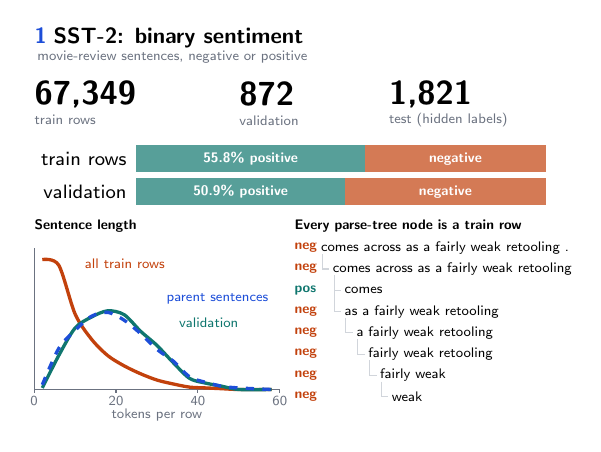
\begin{tikzpicture}[x=1cm,y=1cm]
  \node[ttl] at (0,0.3) {\num{1}SST-2: binary sentiment};
  \node[note,anchor=west] at (0,0.12) {movie-review sentences, negative or positive};
  % split sizes
  \foreach \x/\v/\t in {0/{67,349}/train rows, 2.6/872/validation, 4.5/{1,821}/test (hidden labels)}{
    \node[anchor=west,inner sep=0,font=\large\bfseries] at (\x,-0.35) {\v};
    \node[note,anchor=west,inner sep=0] at (\x,-0.68) {\t};}
  % label balance
  \foreach \y/\n/\p/\pp in {-1.0/train rows/0.558/55.8, -1.42/validation/0.509/50.9}{
    \node[anchor=east,inner sep=2pt] at (1.25,{\y-0.17}) {\n};
    \fill[pos!70] (1.3,\y) rectangle ({1.3+\p*5.2},{\y-0.34});
    \fill[neg!70] ({1.3+\p*5.2},\y) rectangle (6.5,{\y-0.34});
    \node[text=white,font=\tiny\bfseries] at ({1.3+\p*2.6},{\y-0.17}) {\pp\% positive};
    \node[text=white,font=\tiny\bfseries] at ({1.3+\p*5.2+(1-\p)*2.6},{\y-0.17}) {negative};}
  % sentence length (left half)
  \def\b{-4.1}
  \node[anchor=west,inner sep=0,font=\tiny\bfseries] at (0,-2.02) {Sentence length};
  \begin{scope}[xscale=0.52]
    \draw[muted] (0,\b) -- (6.0,\b); \draw[muted] (0,\b) -- (0,{\b+1.8});
    \foreach \t in {0,20,40,60}{\draw[muted] (\t*0.1,\b) -- ++(0,-0.05); \node[note,below] at (\t*0.1,{\b-0.05}) {\t};}
    \draw[neg,very thick] plot[smooth] coordinates {(0.2,{\b+1.65}) (0.6,{\b+1.58}) (1.0,{\b+0.96}) (1.4,{\b+0.64}) (1.8,{\b+0.43}) (2.2,{\b+0.30}) (2.6,{\b+0.20}) (3.0,{\b+0.12}) (3.4,{\b+0.07}) (3.8,{\b+0.03}) (4.2,{\b+0.02}) (4.6,{\b+0.01}) (5.0,\b) (5.8,\b)};
    \draw[color=pos,very thick] plot[smooth] coordinates {(0.2,{\b+0.02}) (0.6,{\b+0.43}) (1.0,{\b+0.78}) (1.4,{\b+0.92}) (1.8,{\b+1.00}) (2.2,{\b+0.95}) (2.6,{\b+0.74}) (3.0,{\b+0.56}) (3.4,{\b+0.34}) (3.8,{\b+0.14}) (4.2,{\b+0.08}) (4.6,{\b+0.04}) (5.0,\b) (5.8,\b)};
    \draw[accent,very thick,dashed] plot[smooth] coordinates {(0.2,{\b+0.06}) (0.6,{\b+0.52}) (1.0,{\b+0.75}) (1.4,{\b+0.93}) (1.8,{\b+0.98}) (2.2,{\b+0.88}) (2.6,{\b+0.71}) (3.0,{\b+0.51}) (3.4,{\b+0.36}) (3.8,{\b+0.16}) (4.2,{\b+0.09}) (4.6,{\b+0.04}) (5.0,{\b+0.02}) (5.8,\b)};
    \node[anchor=west,text=neg,font=\tiny] at (1.0,{\b+1.6}) {all train rows};
    \node[anchor=west,text=accent,font=\tiny] at (3.0,{\b+1.15}) {parent sentences};
    \node[anchor=west,text=pos,font=\tiny] at (3.3,{\b+0.85}) {validation};
    \node[note,below] at (3.0,{\b-0.2}) {tokens per row};
  \end{scope}
  % one train sentence and its sub-phrases (right half): every line is a train row
  \node[anchor=west,inner sep=0,font=\tiny\bfseries] at (3.3,-2.02) {Every parse-tree node is a train row};
  \def\dy{0.27}
  \foreach \i/\l/\t in {
      0/0/comes across as a fairly weak retooling .,
      1/1/comes across as a fairly weak retooling,
      2/2/comes,
      3/2/as a fairly weak retooling,
      4/3/a fairly weak retooling,
      5/4/fairly weak retooling,
      6/5/fairly weak,
      7/6/weak}{
    \node[anchor=west,inner sep=0.5pt,font=\tiny] at ({3.62+0.15*\l},{-2.3-\dy*\i}) {\t};
    \node[anchor=west,inner sep=0,font=\tiny\bfseries,text=neg] at (3.3,{-2.3-\dy*\i}) {\ifnum\i=2\textcolor{pos}{pos}\else neg\fi};}
  \foreach \p/\pl/\c/\cl in {0/0/1/1, 1/1/2/2, 1/1/3/2, 3/2/4/3, 4/3/5/4, 5/4/6/5, 6/5/7/6}{
    \draw[rule] ({3.66+0.15*\pl},{-2.3-\dy*\p-0.08}) |- ({3.6+0.15*\cl},{-2.3-\dy*\c});}
\end{tikzpicture}
\end{column}

\begin{column}{0.47\textwidth}
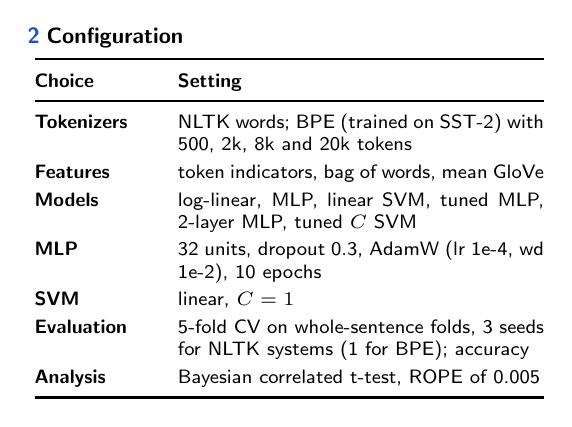
\begin{tikzpicture}[x=1cm,y=1cm]
  \node[ttl] at (0,0.3) {\num{2}Configuration};
  \node[anchor=north west,inner sep=0] at (0,0.12) {\scriptsize
    \renewcommand{\arraystretch}{1.25}
    \begin{tabular}{@{}>{\bfseries}p{1.4cm}p{4.65cm}@{}}
      \toprule
      Choice & \textbf{Setting}\\
      \midrule
      Tokenizers & NLTK words; BPE (trained on SST-2) with 500, 2k, 8k and 20k tokens\\
      Features & token indicators, bag of words, mean GloVe\\
      Models & log-linear, MLP, linear SVM, tuned MLP, 2-layer MLP, tuned $C$ SVM\\
      MLP & 32 units, dropout 0.3, AdamW (lr 1e-4, wd 1e-2), 10 epochs\\
      SVM & linear, $C=1$\\
      Evaluation & 5-fold CV on whole-sentence folds, 3 seeds for NLTK systems (1 for BPE); accuracy\\
      Analysis & Bayesian correlated t-test, ROPE of 0.005\\
      \bottomrule
    \end{tabular}};
\end{tikzpicture}
\end{column}
\end{columns}
\takeaway{Train is 6,885 sentences with their sub-phrases; 77\% share the sentence's label \tsep Validation is balanced, so accuracy is a valid metric (baseline 0.509) \tsep 371 duplicate rows, 5 conflicting labels, no overlap with validation}
\end{frame}

% =====================================================================
% 2  TOKENIZATION
% =====================================================================
\begin{frame}{Tokenization}
\begin{columns}[T]
\begin{column}{0.49\textwidth}
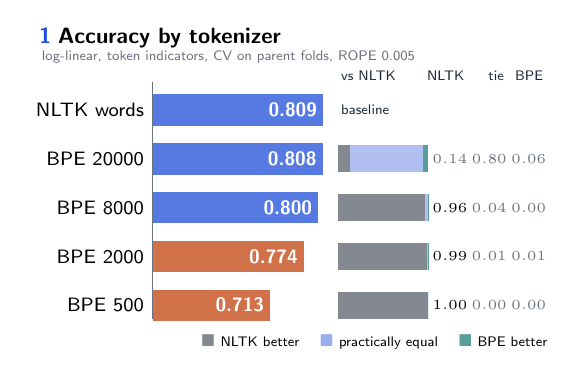
\begin{tikzpicture}[x=1cm,y=1cm]
  \node[ttl] at (-1.45,0.3) {\num{1}Accuracy by tokenizer};
  \node[note,anchor=west] at (-1.45,0.12) {log-linear, token indicators, CV on parent folds, ROPE 0.005};
  \node[note,text=ink,anchor=west] at (2.35,-0.12) {vs NLTK};
  \foreach \x/\t in {4.0/NLTK, 4.5/tie, 5.0/BPE}{\node[note,text=ink,anchor=east] at (\x,-0.12) {\t};}
  \def\s{7.0}
  \foreach \i/\t/\v/\c/\pa/\pt in {0/NLTK words/0.809/accent/0/0, 1/BPE 20000/0.808/accent/0.136/0.800, 2/BPE 8000/0.800/accent/0.961/0.038, 3/BPE 2000/0.774/neg/0.985/0.009, 4/BPE 500/0.713/neg/1.0/0.0}{
    \pgfmathsetmacro{\y}{-0.55-\i*0.62}
    \fill[\c!75] (0,{\y+0.2}) rectangle ({(\v-0.5)*\s},{\y-0.2});
    \node[anchor=east,inner sep=3pt] at (0,\y) {\t};
    \node[anchor=east,inner sep=2pt,font=\scriptsize\bfseries,text=white] at ({(\v-0.5)*\s},\y) {\v};
    \ifnum\i=0
      \node[note,text=ink,anchor=west] at (2.35,\y) {baseline};
    \else
      \postbar{2.35}{\y}{1.15}{0.17}{\pa}{\pt}
      \pnums{4.0}{\y}{0.5}{\pa}{\pt}{\tiny}
    \fi}
  \draw[muted] (0,-0.2) -- (0,-3.2);
  \node[anchor=west,inner sep=0,font=\tiny] at (0.6,-3.5) {\textcolor{ink!55}{$\blacksquare$} NLTK better \quad \textcolor{accent!45}{$\blacksquare$} practically equal \quad \textcolor{pos!70}{$\blacksquare$} BPE better};
\end{tikzpicture}
\end{column}

\begin{column}{0.47\textwidth}
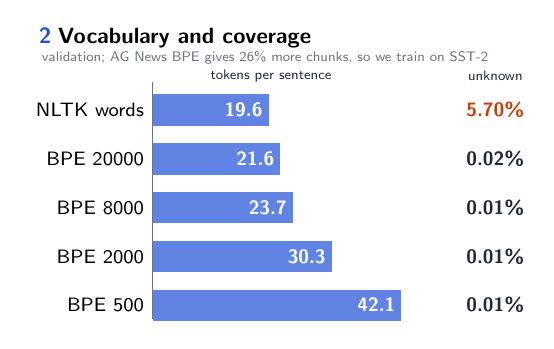
\begin{tikzpicture}[x=1cm,y=1cm]
  \node[ttl] at (-1.45,0.3) {\num{2}Vocabulary and coverage};
  \node[note,anchor=west] at (-1.45,0.12) {validation; AG News BPE gives 26\% more chunks, so we train on SST-2};
  \node[note,text=ink] at (1.5,-0.12) {tokens per sentence};
  \node[note,text=ink] at (4.35,-0.12) {unknown};
  \def\k{0.075}
  \foreach \i/\t/\n/\v/\u/\c in {0/NLTK words/{14,801}/19.6/5.70\%/neg, 1/BPE 20000/{20,000}/21.6/0.02\%/ink, 2/BPE 8000/{8,000}/23.7/0.01\%/ink, 3/BPE 2000/{2,000}/30.3/0.01\%/ink, 4/BPE 500/500/42.1/0.01\%/ink}{
    \pgfmathsetmacro{\y}{-0.55-\i*0.62}
    \fill[accent!70] (0,{\y+0.2}) rectangle ({\v*\k},{\y-0.2});
    \node[anchor=east,inner sep=3pt] at (0,\y) {\t};
    \node[anchor=east,inner sep=2pt,font=\scriptsize\bfseries,text=white] at ({\v*\k},\y) {\v};
    \node[inner sep=0,font=\scriptsize\bfseries,text=\c] at (4.35,\y) {\u};}
  \draw[muted] (0,-0.2) -- (0,-3.2);
\end{tikzpicture}
\end{column}
\end{columns}
\takeaway{BPE 20000 is almost the same as NLTK \tsep BPE 500, 2000 and 8000 are worse than NLTK \tsep We use NLTK}
\end{frame}

% =====================================================================
% 3  REPRESENTATIONS
% =====================================================================
\begin{frame}{Representations: indicators, counts and GloVe}
\begin{center}
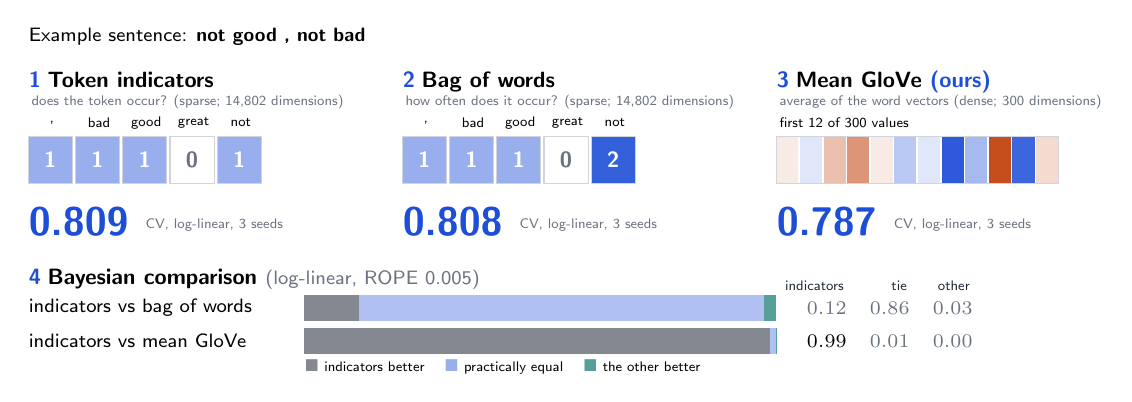
\begin{tikzpicture}[x=1cm,y=1cm]
  \def\cw{0.6}
  \node[anchor=west,inner sep=0] at (0,0.95) {Example sentence: \textbf{\emph{not good , not bad}}};
  % ---- token indicators and bag of words ----
  \foreach \ox/\n/\ttl/\sub/\acc/\vals in {0/1/Token indicators/{does the token occur? (sparse; 14,802 dimensions)}/0.809/{1,1,1,0,1}, 4.75/2/Bag of words/{how often does it occur? (sparse; 14,802 dimensions)}/0.808/{1,1,1,0,2}}{
    \node[ttl] at (\ox,0.3) {\num{\n}\ttl};
    \node[note,anchor=west] at (\ox,0.12) {\sub};
    \foreach \tok [count=\c from 0] in {{,},bad,good,great,not}{
      \node[font=\tiny,inner sep=1pt] at ({\ox+(\c+0.5)*\cw},-0.15) {\tok};}
    \foreach \v [count=\c from 0] in \vals {
      \pgfmathsetmacro{\shade}{min(\v*45,90)}
      \fill[accent!\shade] ({\ox+\c*\cw},-0.32) rectangle ++(\cw-0.04,-0.6);
      \draw[rule] ({\ox+\c*\cw},-0.32) rectangle ++(\cw-0.04,-0.6);
      \pgfmathparse{\v>0 ? 1 : 0}
      \ifnum\pgfmathresult=1
        \node[font=\footnotesize\bfseries,text=white] at ({\ox+(\c+0.5)*\cw-0.02},-0.62) {\v};
      \else
        \node[font=\footnotesize\bfseries,text=muted] at ({\ox+(\c+0.5)*\cw-0.02},-0.62) {\v};
      \fi}
    \node[anchor=west,inner sep=0,font=\Large\bfseries,text=accent] at (\ox,-1.4) {\acc};
    \node[note,anchor=west] at ({\ox+1.45},-1.45) {CV, log-linear, 3 seeds};}
  % ---- mean GloVe ----
  \def\ox{9.5}
  \node[ttl] at (\ox,0.3) {\num{3}Mean GloVe \textcolor{accent}{(ours)}};
  \node[note,anchor=west] at (\ox,0.12) {average of the word vectors (dense; 300 dimensions)};
  \node[font=\tiny,inner sep=1pt,anchor=west] at (\ox,-0.15) {first 12 of 300 values};
  \foreach \v [count=\c from 0] in {-0.01,0.02,-0.09,-0.17,-0.01,0.08,0.02,0.34,0.11,-1.97,0.28,-0.04}{
    \pgfmathsetmacro{\shade}{min(abs(\v)*280,85)+8}
    \pgfmathparse{\v>0 ? 1 : 0}
    \ifnum\pgfmathresult=1
      \fill[accent!\shade] ({\ox+\c*0.3},-0.32) rectangle ++(0.28,-0.6);
    \else
      \fill[neg!\shade] ({\ox+\c*0.3},-0.32) rectangle ++(0.28,-0.6);
    \fi}
  \draw[rule] (\ox,-0.32) rectangle ++(3.58,-0.6);
  \node[anchor=west,inner sep=0,font=\Large\bfseries,text=accent] at (\ox,-1.4) {0.787};
  \node[note,anchor=west] at ({\ox+1.45},-1.45) {CV, log-linear, 3 seeds};
  % ---- comparison ----
  \node[ttl] at (0,-2.2) {\num{4}Bayesian comparison \lab{\scriptsize\mdseries(log-linear, ROPE 0.005)}};
  \foreach \i/\t/\pa/\pt in {0/indicators vs bag of words/0.116/0.857, 1/indicators vs mean GloVe/0.986/0.013}{
    \pgfmathsetmacro{\y}{-2.5-\i*0.42}
    \node[anchor=west,inner sep=0] at (0,\y) {\t};
    \postbar{3.5}{\y}{6.0}{0.16}{\pa}{\pt}
    \pnums{10.4}{\y}{0.8}{\pa}{\pt}{\scriptsize}}
  \foreach \x/\t in {10.4/indicators, 11.2/tie, 12.0/other}{\node[note,text=ink,anchor=east] at (\x,-2.22) {\t};}
  \node[anchor=west,inner sep=0,font=\tiny] at (3.5,-3.25) {\textcolor{ink!55}{$\blacksquare$} indicators better \quad \textcolor{accent!45}{$\blacksquare$} practically equal \quad \textcolor{pos!70}{$\blacksquare$} the other better};
\end{tikzpicture}
\end{center}
\takeaway{Indicators and bag of words are practically equivalent: only 7.3\% of features have a count above 1 \tsep Mean GloVe is worse: averaging loses word order \tsep Considered but not tried: TF-IDF, n-grams, a learned embedding layer}
\end{frame}

% =====================================================================
% 4  ARCHITECTURES
% =====================================================================
\begin{frame}{Architectures: log-linear, MLP and linear SVM}
\begin{columns}[T]
\begin{column}{0.49\textwidth}
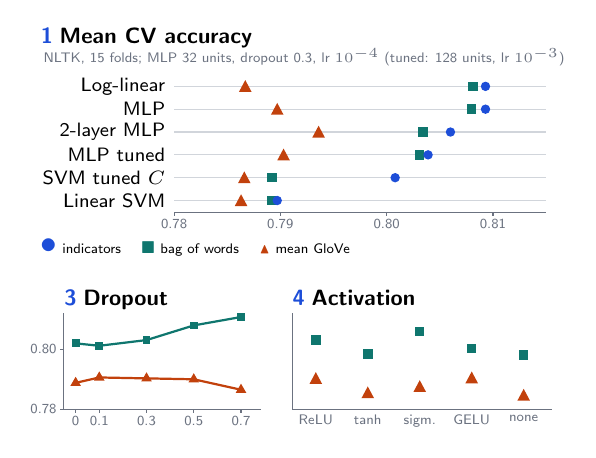
\begin{tikzpicture}[x=1cm,y=1cm]
  \node[ttl] at (-1.7,0.3) {\num{1}Mean CV accuracy};
  \node[note,anchor=west] at (-1.7,0.12) {NLTK, 15 folds; MLP 32 units, dropout 0.3, lr $10^{-4}$ (tuned: 128 units, lr $10^{-3}$)};
  \foreach \i/\n/\a/\b/\g in {0/Log-linear/0.8093/0.8081/0.7867, 1/MLP/0.8093/0.8080/0.7897, 2/2-layer MLP/0.8060/0.8034/0.7936, 3/MLP tuned/0.8039/0.8031/0.7903, 4/SVM tuned $C$/0.8008/0.7892/0.7866, 5/Linear SVM/0.7897/0.7892/0.7863}{
    \pgfmathsetmacro{\y}{-0.25-\i*0.29}
    \node[anchor=east,inner sep=3pt] at (0,\y) {\n};
    \draw[rule] (0,\y) -- ({\xc{0.815}},\y);
    \fill[neg] ({\xc{\g}},\y) ++(0,0.08) -- ++(0.08,-0.15) -- ++(-0.16,0) -- cycle;
    \fill[color=pos] ({\xc{\b}-0.06},\y-0.06) rectangle ++(0.12,0.12);
    \fill[accent] ({\xc{\a}},\y) circle (1.7pt);}
  \draw[muted] (0,-1.85) -- ({\xc{0.815}},-1.85);
  \foreach \a in {0.78,0.79,0.80,0.81}{\draw[muted] ({\xc{\a}},-1.85) -- ++(0,-0.05); \node[note,below] at ({\xc{\a}},-1.9) {\a};}
  \node[anchor=west,inner sep=0,font=\tiny] at (-1.7,-2.3) {\textcolor{accent}{\large$\bullet$} indicators \quad \textcolor{pos}{$\blacksquare$} bag of words \quad \textcolor{neg}{$\blacktriangle$} mean GloVe};
  % ---- dropout ----
  \begin{scope}[shift={(-1.4,-4.35)}]
    \node[ttl] at (0,1.32) {\num{3}Dropout};
    \draw[muted] (0,0) -- (2.5,0); \draw[muted] (0,0) -- (0,1.22);
    \foreach \a in {0.78,0.80}{\draw[muted] (0,{\yd{\a}}) -- ++(-0.05,0); \node[note,left] at (-0.05,{\yd{\a}}) {\a};}
    \foreach \d in {0,0.1,0.3,0.5,0.7}{\draw[muted] ({\d*3+0.15},0) -- ++(0,-0.05); \node[note,below] at ({\d*3+0.15},-0.05) {\d};}
    \draw[color=pos,thick] plot[mark=square*,mark size=1.0pt] coordinates {(0.15,{\yd{0.8020}}) (0.45,{\yd{0.8012}}) (1.05,{\yd{0.8031}}) (1.65,{\yd{0.8080}}) (2.25,{\yd{0.8108}})};
    \draw[neg,thick] plot[mark=triangle*,mark size=1.4pt] coordinates {(0.15,{\yd{0.7888}}) (0.45,{\yd{0.7906}}) (1.05,{\yd{0.7903}}) (1.65,{\yd{0.7900}}) (2.25,{\yd{0.7865}})};
  \end{scope}
  % ---- activation ----
  \begin{scope}[shift={(1.5,-4.35)}]
    \node[ttl] at (0,1.32) {\num{4}Activation};
    \draw[muted] (0,0) -- (3.3,0); \draw[muted] (0,0) -- (0,1.22);
    \foreach \i/\n/\bw/\g in {0/ReLU/0.8031/0.7903, 1/tanh/0.7985/0.7855, 2/sigm./0.8060/0.7876, 3/GELU/0.8003/0.7905, 4/none/0.7981/0.7847}{
      \pgfmathsetmacro{\x}{0.3+\i*0.66}
      \fill[color=pos] (\x-0.06,{\yd{\bw}-0.06}) rectangle ++(0.12,0.12);
      \fill[neg] (\x,{\yd{\g}}) ++(0,0.08) -- ++(0.08,-0.15) -- ++(-0.16,0) -- cycle;
      \node[note,below] at (\x,-0.03) {\n};}
  \end{scope}
\end{tikzpicture}
\end{column}

\begin{column}{0.47\textwidth}
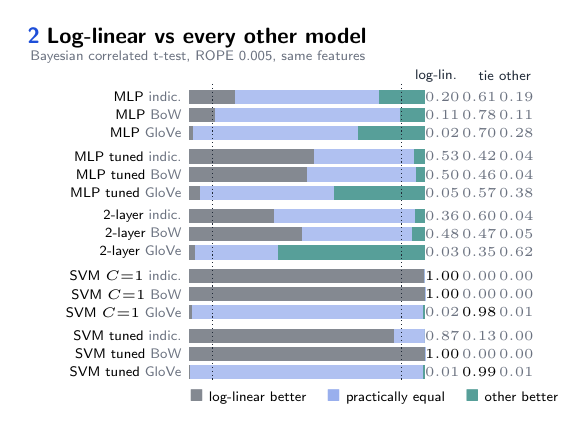
\begin{tikzpicture}[x=1cm,y=1cm]
  \node[ttl] at (0,0.3) {\num{2}Log-linear vs every other model};
  \node[note,anchor=west] at (0,0.12) {Bayesian correlated t-test, ROPE 0.005, same features};
  \def\bx{2.05}
  \def\bw{3.0}
  \pgfmathsetmacro{\yy}{0}
  \foreach \i/\t/\pa/\pt/\f in {
     0/MLP/0.195/0.610/indic., 1/MLP/0.113/0.782/BoW, 2/MLP/0.017/0.699/GloVe,
     3/MLP tuned/0.532/0.424/indic., 4/MLP tuned/0.503/0.460/BoW, 5/MLP tuned/0.050/0.567/GloVe,
     6/2-layer/0.362/0.597/indic., 7/2-layer/0.479/0.469/BoW, 8/2-layer/0.029/0.348/GloVe,
     9/SVM $C{=}1$/0.998/0.002/indic., 10/SVM $C{=}1$/0.999/0.001/BoW, 11/SVM $C{=}1$/0.016/0.977/GloVe,
     12/SVM tuned/0.870/0.130/indic., 13/SVM tuned/0.999/0.001/BoW, 14/SVM tuned/0.008/0.985/GloVe}{
    \pgfmathtruncatemacro{\grp}{int(\i/3)}
    \pgfmathsetmacro{\y}{-0.38-\i*0.23-\grp*0.07}
    \node[anchor=east,inner sep=1.5pt,font=\tiny] at ({\bx-0.03},\y) {\t\ \lab{\f}};
    \postbar{\bx}{\y}{\bw}{0.09}{\pa}{\pt}
    \pnums{5.5}{\y}{0.47}{\pa}{\pt}{\tiny}}
  \foreach \x/\t in {5.5/log-lin., 5.97/tie, 6.44/other}{\node[note,text=ink,anchor=east] at (\x,-0.12) {\t};}
  \draw[ink,densely dotted] ({\bx+0.9*\bw},-0.22) -- ({\bx+0.9*\bw},-4.0);
  \draw[ink,densely dotted] ({\bx+0.1*\bw},-0.22) -- ({\bx+0.1*\bw},-4.0);
  \node[anchor=west,inner sep=0,font=\tiny] at (\bx,-4.2) {\textcolor{ink!55}{$\blacksquare$} log-linear better \quad \textcolor{accent!45}{$\blacksquare$} practically equal \quad \textcolor{pos!70}{$\blacksquare$} other better};
\end{tikzpicture}
\end{column}
\end{columns}
\takeaway{A hidden layer gives no evidence of improvement \tsep Tuning the MLP or adding a second layer gives no reliable gain \tsep Log-linear beats the $C{=}1$ SVM on indicators and bag of words; tuning $C$ on indicators lifts it from 0.790 to 0.801 ($P=0.94$)}
\end{frame}

% =====================================================================
% 5  EVALUATION
% =====================================================================
\begin{frame}{Evaluation: cross-validation without leakage}
\begin{columns}[T]
\begin{column}{0.51\textwidth}
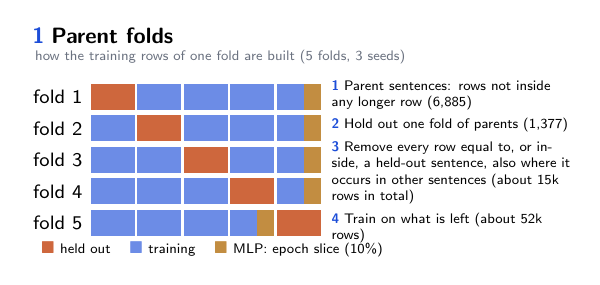
\begin{tikzpicture}[x=1cm,y=1cm]
  \node[ttl] at (0,0.3) {\num{1}Parent folds};
  \node[note,anchor=west] at (0,0.12) {how the training rows of one fold are built (5 folds, 3 seeds)};
  \def\bw{0.56}   % block width
  \def\bh{0.33}   % block height
  \foreach \f in {0,...,4}{
    \pgfmathsetmacro{\y}{-0.22-\f*0.4}
    \pgfmathtruncatemacro{\ff}{\f+1}
    \node[anchor=east,inner sep=2pt] at (0.72,{\y-\bh/2}) {fold \ff};
    \foreach \c in {0,...,4}{
      \pgfmathsetmacro{\x}{0.75+\c*(\bw+0.03)}
      \ifnum\c=\f
        \fill[neg!80] (\x,\y) rectangle ({\x+\bw},{\y-\bh});
      \else
        \fill[accent!65] (\x,\y) rectangle ({\x+\bw},{\y-\bh});
      \fi}
    % inner validation slice: 10% of the training part, at the end of the row
    \pgfmathsetmacro{\e}{0.75+(\f==4 ? 4 : 5)*(\bw+0.03)-0.03}
    \fill[amber!85] ({\e-0.22},\y) rectangle (\e,{\y-\bh});}
  \node[anchor=west,inner sep=0,font=\tiny] at (0.1,-2.32) {\textcolor{neg!80}{$\blacksquare$} held out \;\; \textcolor{accent!65}{$\blacksquare$} training \;\; \textcolor{amber!85}{$\blacksquare$} MLP: epoch slice (10\%)};
  % how the rows are constructed
  \node[anchor=north west,inner sep=0,text width=3.05cm,align=left,font=\tiny] at (3.8,-0.17) {%
    \textbf{\textcolor{accent}{1}} Parent sentences: rows not inside any longer row (6,885)\\[2pt]
    \textbf{\textcolor{accent}{2}} Hold out one fold of parents (1,377)\\[2pt]
    \textbf{\textcolor{accent}{3}} Remove every row equal to, or inside, a held-out sentence, also where it occurs in other sentences (about 15k rows in total)\\[2pt]
    \textbf{\textcolor{accent}{4}} Train on what is left (about 52k rows)};
\end{tikzpicture}
\end{column}

\begin{column}{0.45\textwidth}
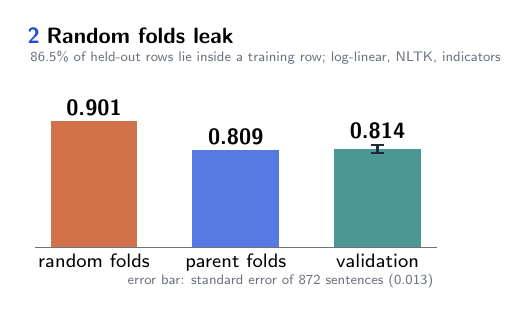
\begin{tikzpicture}[x=1cm,y=1cm]
  \node[ttl] at (0,0.3) {\num{2}Random folds leak};
  \node[note,anchor=west] at (0,0.12) {86.5\% of held-out rows lie inside a training row; log-linear, NLTK, indicators};
  \def\b{-2.3}
  \def\s{4.0}
  \foreach \x/\v/\c/\t in {0.85/0.901/neg/random folds, 2.65/0.809/accent/parent folds, 4.45/0.814/pos/validation}{
    \fill[\c!75] (\x-0.55,\b) rectangle (\x+0.55,{\b+(\v-0.5)*\s});
    \node[below,inner sep=2pt] at (\x,\b) {\t};}
  \foreach \x/\v in {0.85/0.901, 2.65/0.809}{\node[above,inner sep=2pt,font=\footnotesize\bfseries] at (\x,{\b+(\v-0.5)*\s}) {\v};}
  % standard error of 872 sentences on the validation bar
  \draw[ink,thick] (4.45,{\b+(0.814-0.013-0.5)*\s}) -- (4.45,{\b+(0.814+0.013-0.5)*\s});
  \draw[ink,thick] (4.37,{\b+(0.814+0.013-0.5)*\s}) -- (4.53,{\b+(0.814+0.013-0.5)*\s});
  \draw[ink,thick] (4.37,{\b+(0.814-0.013-0.5)*\s}) -- (4.53,{\b+(0.814-0.013-0.5)*\s});
  \node[above,inner sep=2pt,font=\footnotesize\bfseries] at (4.45,{\b+(0.814+0.013-0.5)*\s}) {0.814};
  \draw[muted] (0.1,\b) -- (5.2,\b);
  \node[note,anchor=east] at (5.2,{\b-0.42}) {error bar: standard error of 872 sentences (0.013)};
\end{tikzpicture}
\end{column}
\end{columns}
\par\vspace{0.5mm}
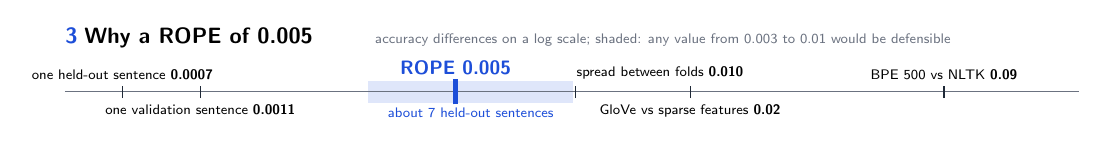
\begin{tikzpicture}[x=1cm,y=1cm]
  \node[ttl] at (0,0.62) {\num{3}Why a ROPE of 0.005};
  \node[note,anchor=west] at (3.9,0.66) {accuracy differences on a log scale; shaded: any value from 0.003 to 0.01 would be defensible};
  % every value between 0.003 and 0.01 is defensible
  \fill[accent!14] ({\xl{0.003}},0.14) rectangle ({\xl{0.01}},-0.14);
  \draw[muted] (0,0) -- ({\xl{0.2}},0);
  \foreach \v/\t/\u/\up in {
      0.0007/one held-out sentence/0.0007/1,
      0.0011/one validation sentence/0.0011/0,
      0.02/GloVe vs sparse features/0.02/0,
      0.09/BPE 500 vs NLTK/0.09/1}{
    \draw[ink] ({\xl{\v}},-0.08) -- ({\xl{\v}},0.08);
    \ifnum\up=1
      \node[anchor=south,inner sep=1.5pt,font=\tiny,align=center] at ({\xl{\v}},0.1) {\t\ \textbf{\u}};
    \else
      \node[anchor=north,inner sep=1.5pt,font=\tiny,align=center] at ({\xl{\v}},-0.1) {\t\ \textbf{\u}};
    \fi}
  \draw[ink] ({\xl{0.0102}},-0.08) -- ({\xl{0.0102}},0.08);
  \node[anchor=south west,inner sep=1.5pt,font=\tiny] at ({\xl{0.0102}-0.05},0.1) {spread between folds \textbf{0.010}};
  \draw[accent,line width=1.6pt] ({\xl{0.005}},-0.16) -- ({\xl{0.005}},0.16);
  \node[anchor=south,inner sep=1.5pt,font=\scriptsize\bfseries,text=accent] at ({\xl{0.005}},0.16) {ROPE 0.005};
  \node[anchor=north,inner sep=1.5pt,font=\tiny,text=accent] at ({\xl{0.0055}},-0.14) {about 7 held-out sentences};
\end{tikzpicture}
\takeaway{Random folds give higher CV accuracy through leakage \tsep 3 seeds $\times$ 5 folds = 15 paired scores \tsep Building the tokenizer on all of train causes no inflation (per-fold vocabulary changes at most 0.003)}
\end{frame}

% =====================================================================
% 6  ANALYSIS AND CHOICE
% =====================================================================
\begin{frame}{Analysis and choice}
\begin{center}
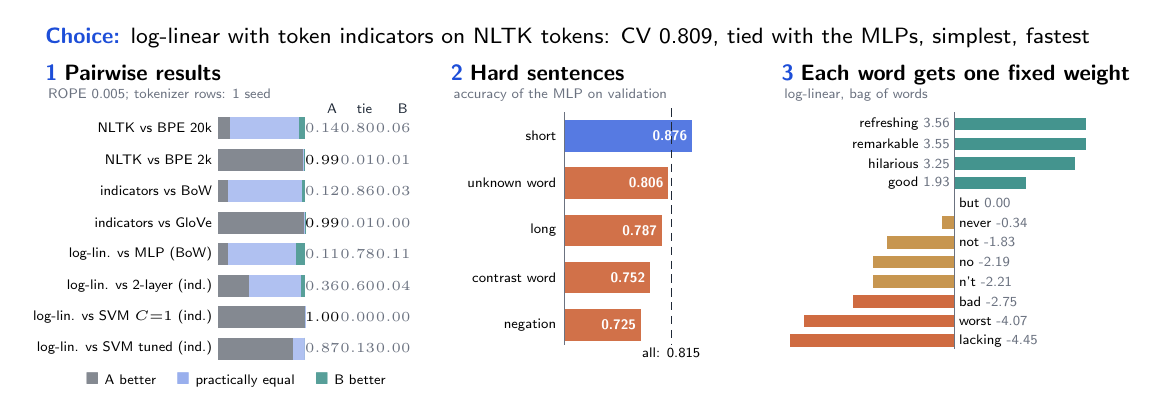
\begin{tikzpicture}[x=1cm,y=1cm]
  \node[anchor=west,inner sep=0,font=\footnotesize] at (0,0.85) {\textbf{\textcolor{accent}{Choice:}} log-linear with token indicators on NLTK tokens: CV 0.809, tied with the MLPs, simplest, fastest};
  % ---- pairwise results ----
  \node[ttl] at (0,0.3) {\num{1}Pairwise results};
  \node[note,anchor=west] at (0,0.12) {ROPE 0.005; tokenizer rows: 1 seed};
  \foreach \i/\t/\pa/\pt in {
     0/NLTK vs BPE 20k/0.136/0.800,
     1/NLTK vs BPE 2k/0.985/0.009,
     2/indicators vs BoW/0.116/0.857,
     3/indicators vs GloVe/0.986/0.013,
     4/log-lin. vs MLP (BoW)/0.113/0.782,
     5/log-lin. vs 2-layer (ind.)/0.362/0.597,
     6/log-lin. vs SVM $C{=}1$ (ind.)/0.998/0.002,
     7/log-lin. vs SVM tuned (ind.)/0.870/0.130}{
    \pgfmathsetmacro{\y}{-0.3-\i*0.4}
    \node[anchor=east,inner sep=2pt,font=\tiny] at (2.2,\y) {\t};
    \postbar{2.2}{\y}{1.1}{0.14}{\pa}{\pt}
    \pnums{3.75}{\y}{0.45}{\pa}{\pt}{\tiny}}
  \foreach \x/\t in {3.75/A, 4.2/tie, 4.65/B}{\node[note,text=ink,anchor=east] at (\x,-0.05) {\t};}
  \node[anchor=west,inner sep=0,font=\tiny] at (0.5,-3.5) {\textcolor{ink!55}{$\blacksquare$} A better \quad \textcolor{accent!45}{$\blacksquare$} practically equal \quad \textcolor{pos!70}{$\blacksquare$} B better};
  % ---- hard sentences ----
  \begin{scope}[shift={(6.6,0)}]
    \node[ttl] at (-1.45,0.3) {\num{2}Hard sentences};
    \node[note,anchor=west] at (-1.45,0.12) {accuracy of the MLP on validation};
    \def\s{4.3}
    \def\all{0.815}
    \foreach \i/\t/\v/\col in {0/short/0.876/accent, 1/unknown word/0.806/neg, 2/long/0.787/neg, 3/contrast word/0.752/neg, 4/negation/0.725/neg}{
      \pgfmathsetmacro{\y}{-0.4-\i*0.6}
      \fill[\col!75] (0,{\y+0.2}) rectangle ({(\v-0.5)*\s},{\y-0.2});
      \node[anchor=east,inner sep=2pt,font=\tiny] at (-0.03,\y) {\t};
      \node[anchor=east,inner sep=1.5pt,font=\tiny\bfseries,text=white] at ({(\v-0.5)*\s},\y) {\v};}
    \draw[muted] (0,-0.1) -- (0,-3.05);
    \draw[ink,densely dashed] ({(\all-0.5)*\s},-0.05) -- ({(\all-0.5)*\s},-3.05);
    \node[anchor=north,inner sep=1pt,font=\tiny] at ({(\all-0.5)*\s},-3.05) {all: \all};
  \end{scope}
  % ---- weights ----
  \begin{scope}[shift={(9.35,0)}]
    \node[ttl] at (0,0.3) {\num{3}Each word gets one fixed weight};
    \node[note,anchor=west] at (0,0.12) {log-linear, bag of words};
    \def\c{2.2}
    \def\k{0.47}
    \foreach \i/\word/\v/\col in {
       0/refreshing/3.56/pos, 1/remarkable/3.55/pos, 2/hilarious/3.25/pos, 3/good/1.93/pos,
       4/but/0.00/amber, 5/never/-0.34/amber, 6/not/-1.83/amber, 7/no/-2.19/amber, 8/n't/-2.21/amber,
       9/bad/-2.75/neg, 10/worst/-4.07/neg, 11/lacking/-4.45/neg}{
      \pgfmathsetmacro{\y}{-0.25-\i*0.25}
      \fill[\col!78] (\c,{\y+0.08}) rectangle ({\c+\v*\k},{\y-0.08});
      \pgfmathparse{\v>0 ? 1 : 0}
      \ifnum\pgfmathresult=1
        \node[anchor=east,inner sep=1.5pt,font=\tiny] at (\c,\y) {\word\ \lab{\v}};
      \else
        \node[anchor=west,inner sep=1.5pt,font=\tiny] at (\c,\y) {\word\ \lab{\v}};
      \fi}
    \draw[muted] (\c,-0.1) -- (\c,-3.1);
  \end{scope}
\end{tikzpicture}
\end{center}
\takeaway{No clear winner among log-linear and MLPs on indicators and counts: undecided at ROPE 0.005, practically equivalent at 0.01 \tsep 5 of 6 systems predict 53--55\% positive (50.9\% true) \tsep MLPs are 3--7 times slower, for no gain}
\end{frame}

\end{document}
